\documentclass[12pt]{article}

\usepackage[a4paper,margin=1in]{geometry}
\usepackage[utf8]{inputenc}
\usepackage[spanish,es-tabla]{babel}
\usepackage{graphicx}
\usepackage{circuitikz}
\usepackage{amsmath}
\usepackage{subcaption}
\usepackage{amssymb}
\usepackage[hidelinks]{hyperref}
\usepackage{mathtools}
%\usepackage[table,xcdraw]{xcolor}
\usepackage{enumitem}
\usepackage{array}
\usepackage{longtable}
\usepackage{csquotes}          
\usepackage{float}
\usepackage{setspace}
\usepackage[style=ieee, backend=biber]{biblatex}
\addbibresource{bibliografía.bib}  
\graphicspath{{Figuras/}} 
\onehalfspacing

\hypersetup{
    colorlinks=true,
    linkcolor=blue,    
    citecolor=blue,
    urlcolor=blue,
    filecolor=blue
}

\begin{document}       
\renewcommand{\figureautorefname}{Fig.}
\renewcommand{\tableautorefname}{Tab.}
\renewcommand{\equationautorefname}{Ec.}

\begin{titlepage}
\thispagestyle{empty}
\begin{tikzpicture}[remember picture,overlay]
    \node[opacity=0.2,anchor=center] at (current page.center) 
        {
\includegraphics[width=0.9\paperwidth]{decoracion_a.png}};
\end{tikzpicture}
\begin{center}
    
\includegraphics[width=15cm]{unc_fcefyn_logo.png} \\ [0.5cm]
    \LARGE Universidad Nacional de Córdoba \\ [0.5cm] 
    \large Facultad de Ciencias Exactas, Físicas y Naturales \\ 
    \vspace{40pt}
    \large Sistemas de Radiocomunicación \\ [0.2cm]
    \large Trabajo Práctico N°2 \\
    \vspace{60pt}
    \LARGE Radioenlaces Punto a Punto \\
    \vspace{60pt}
    \begin{table}[!h]
        \centering
        \begin{tabular}{ll}
            \multicolumn{1}{c}{Nombre} & \multicolumn{1}{c}{DNI} \\
            Mendes Rosa, Agustín             & 44.517.201 \\
            Monja, Ernesto Joaquín           & 43.873.728
        \end{tabular}
    \end{table}
    \vspace{20pt}
    \begin{table}[!h]
        \centering
        \begin{tabular}{ll}
            \multicolumn{1}{c}{Docentes} & Esp. Ing. Liendo, Carlos Guillermo \\
                                         & Ing. Dadam, Federico Tomás \\
        \end{tabular}
    \end{table}
    \vfill
        {\small Córdoba, República Argentina\\
                Año 2026}
\end{center}
\end{titlepage}
\newpage

\tableofcontents
\newpage



\section{Introducción}
\label{sec_1}
...



\section{Parte 1 - Diseño y simulación de un enlace radioeléctrico punto a punto}
\label{sec_2}
\subsection{Introducción Teórica}
\label{sec_2.1}
Un radioenlace es un sistema de interconexión entre terminales de telecomunicación que utiliza la propagación de ondas electromagnéticas a través del espectro radioeléctrico, operando por lo general en frecuencias entre $800 \, [MHz]$ y $50 \, [GHz]$. \cite{b1}


\subsubsection{Principales componentes de un enlace radioeléctrico punto a punto}
\label{sec_2.1.1}
De acuerdo a los lineamientos de diseño de radioenlaces y la infraestructura necesaria, los principales componentes son:
\begin{enumerate}
    \item \underline{Transceptor (Equipos de radio):} Son los terminales de telecomunicación encargados de procesar, modular y transmitir la señal, así como de recibirla y de-modularla en el extremo opuesto.
    \item \underline{Antena:} Es el elemento que extrae potencia del frente de onda electromagnético incidente o irradia la señal al espacio. En enlaces de microondas se suelen utilizar reflectores parabólicos y antenas bocina (\textit{horns}).
    \item \underline{Torre o mástil:} Es la estructura necesaria para elevar las antenas y asegurar el despeje de la trayectoria. Deben estar preparadas para soportar físicamente el peso y la carga al viento que presentan las antenas y las líneas de transmisión.
    \item \underline{Cableado de datos y de \textit{RF} (líneas de transmisión y guías de onda):} Se utilizan cables coaxiales (flexibles, semirígidos o rígidos) y guías de onda para transportar la señal de radiofrecuencia entre los equipos y las antenas.
    \item \underline{Conectores y bridas:} Permiten la vinculación mecánica y eléctrica de los cables o guías de ondas. Las uniones (como las bridas \textit{EIA} flanges) deben ser precisas para evitar discontinuidades de impedancia y picos de ondas estacionarias (\textit{ROE}).
    \item \underline{Otros componentes de infraestructura:} Para el correcto funcionamiento e interconexión a la red, el sistema incluye típicamente soportes de montaje, sistemas de alimentación y PoE (\textit{Power over Ethernet}) para energizar equipos de exteriores, protecciones contra sobretensiones y sistemas de puesta a tierra para salvaguardar el equipamiento, y cableado de datos o fibra óptica para la vinculación final con la red local.  \cite{b1}
\end{enumerate}


\subsubsection{Principales parámetros que influyen en el comportamiento del enlace}
\label{sec_2.1.2}
Para el correcto diseño y balance de potencias del radioenlace, se deben considerar los siguientes parámetros:
\begin{itemize}
    \item \underline{Frecuencia de operación:} Determina la banda de trabajo (típicamente entre $800 \, [MHz]$ y $50 \, [GHz]$) y afecta directamente cómo se comportará la propagación de la onda, el tamaño de las antenas y guías de onda, y los límites regulatorios.
    \item \underline{Ganancia de antena:} Es la relación entre la máxima intensidad de radiación de la antena y la intensidad de una antena isotrópica teórica. Depende de la directividad y de la eficiencia (apertura efectiva) de la antena.
    \item \underline{Pérdidas en cables y conectores (Atenuación):} Es el decremento gradual de la señal a medida que viaja por la línea de transmisión debido a pérdidas en los conductores y en el dieléctrico. También se incluyen las pérdidas generadas por reflexiones en los conectores.
    \item \underline{Pérdidas de propagación:} Son las atenuaciones sufridas por la señal en el trayecto espacial. Incluyen las pérdidas del espacio libre y pueden agravarse si hay obstrucciones en las \textit{Zonas de Fresnel} de la trayectoria.
    \item \underline{Sensibilidad del receptor:} Es la potencia mínima necesaria en la antena receptora para obtener una relación señal/ruido (\textit{SNR}) suficiente que permita recibir y procesar la señal correctamente (umbral de ruido).
    \item \underline{Nivel de ruido:} Es la potencia de ruido presente en el sistema, generada internamente por el movimiento estocástico de portadores de carga (ruido térmico) en los conductores, o captada por la antena desde fuentes externas.
    \item \underline{Relación señal/ruido (\textit{SNR}):} Es la medida que compara la potencia de la señal recibida frente a la potencia del ruido. Una mejor \textit{SNR} determina la viabilidad del enlace. En los enlaces digitales, la \textit{SNR} impacta en la tasa de errores de bit (\textit{BER}).
    \item \underline{Interferencias:} Son señales provenientes de otros servicios en frecuencias adyacentes o dentro de la misma banda que afectan negativamente la recepción de nuestra señal. Se pueden mitigar mejorando las características de la antena (por ejemplo, utilizando reflectores profundos o ``\textit{deep reflectors}'') o mediante filtros.
    \item \underline{Margen de enlace (Balance de potencias):} Es el análisis completo de la trayectoria del haz que contabiliza la potencia transmitida, las ganancias de las antenas y todas las atenuaciones del camino.
    \item \underline{Ancho de canal, Modulación y \textit{MCS}, Nivel de señal recibida, Capacidad esperada:} Son los parámetros operativos de las radios de telecomunicación. El esquema de modulación y ancho de banda determinan el ``\textit{throughput}'' o capacidad de transporte de datos del enlace, lo cual requiere que el nivel de señal recibida sea lo suficientemente alto respecto a la sensibilidad de ese modo específico. \cite{b1}
\end{itemize}



\subsection{Definición del enlace}
\label{sec_2.2}
El desarrollo y diseño del radioenlace para este trabajo práctico, se basa en el \textbf{Enlace A} propuesto por los docentes de esta asignatura el cual consiste de los siguientes dos puntos:
\begin{figure}[H]
    \centering
    \begin{minipage}{0.48\linewidth}
        \centering
        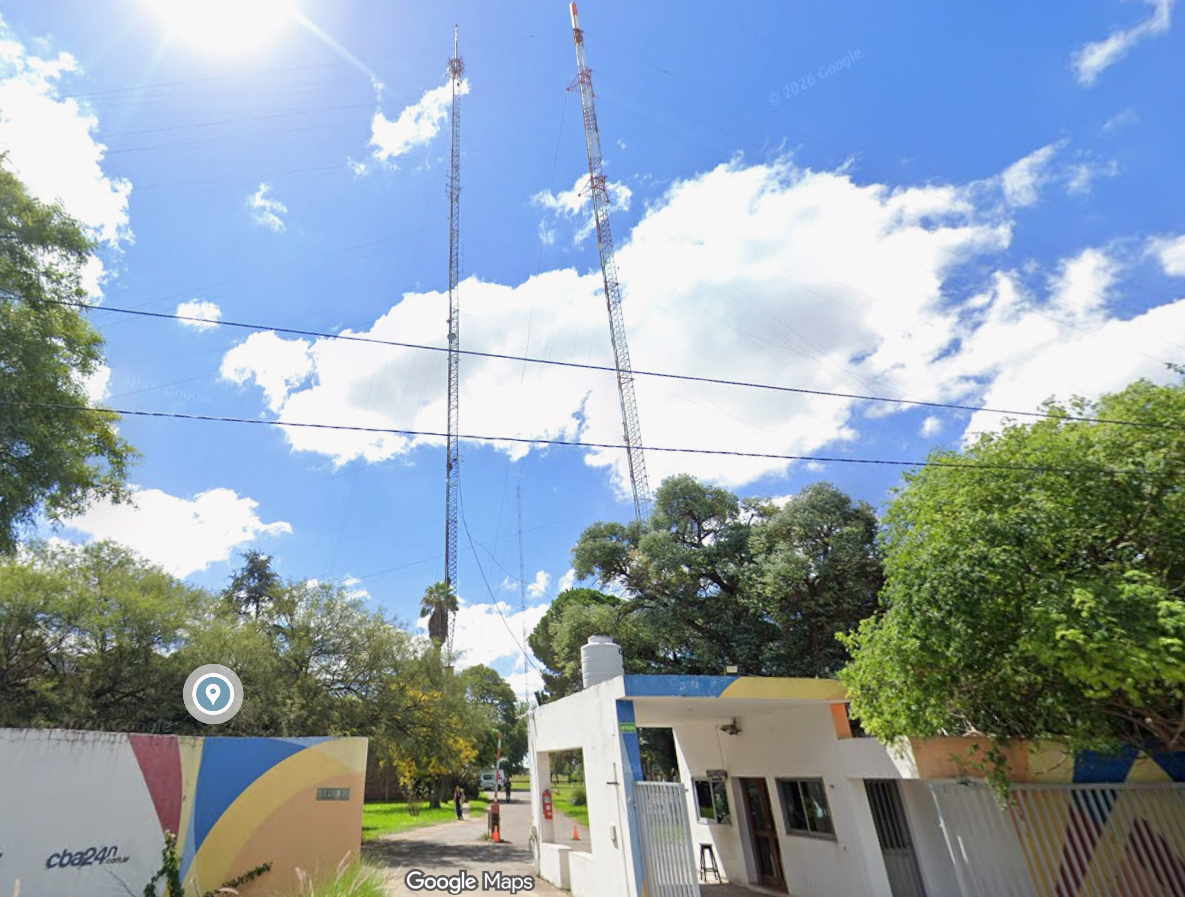
\includegraphics[width=0.86\linewidth]{Figura 1.1.png}
    \end{minipage}
    \hfill
    \begin{minipage}{0.48\linewidth}
        \centering
        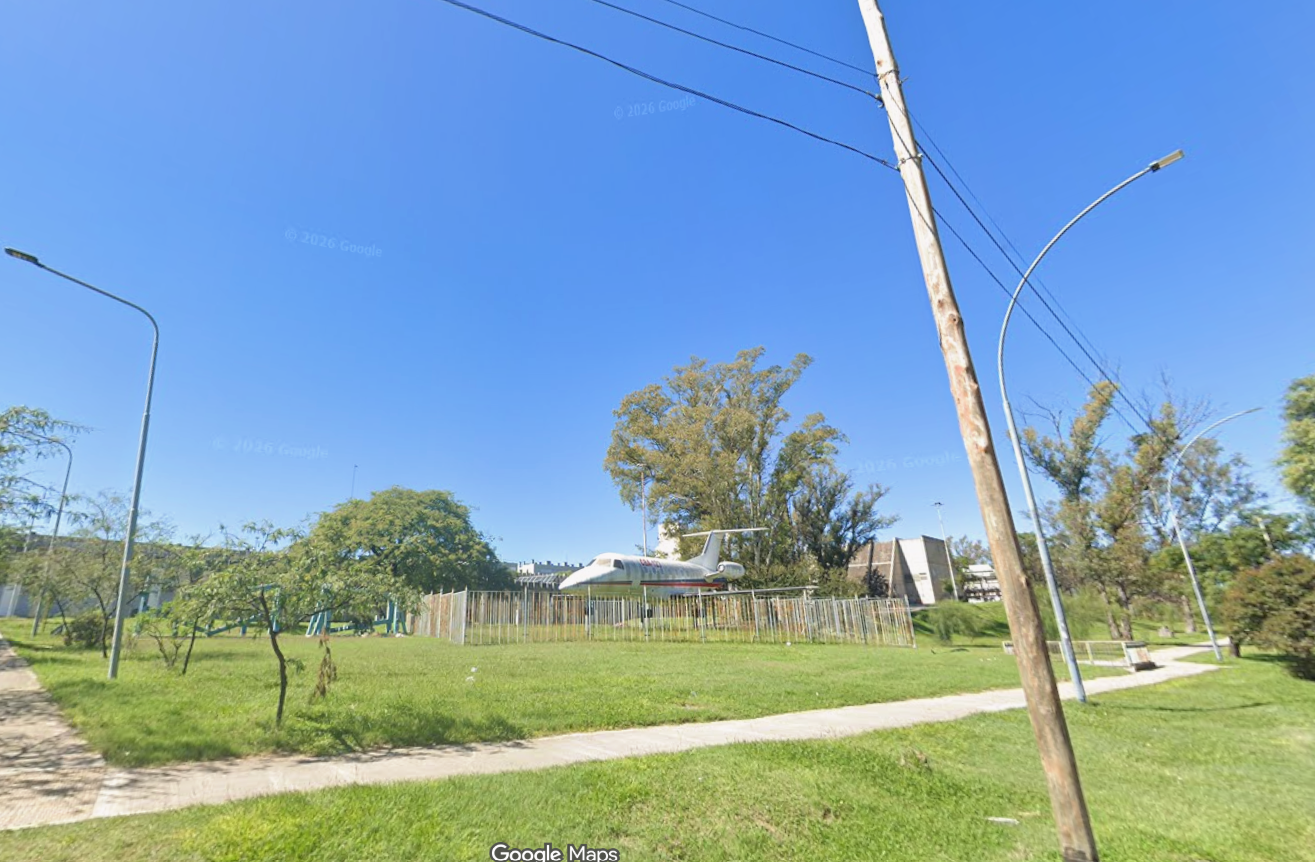
\includegraphics[width=1\linewidth]{Figura 1.2.png}
    \end{minipage}
    \caption{A la izquierda se observa el mástil de Canal 10, mientras que a la derecha se observa el avión instalado en la FCEFyN.}
    \label{fig:fig_1}
\end{figure}

Este radioenlace punto a punto será la base práctica sobre la cual se aplicarán los conceptos teóricos descritos, llevando a cabo el dimensionamiento, la selección de equipamiento, el cálculo del balance de potencias y la evaluación de viabilidad física y radioeléctrica, con el objetivo primordial de garantizar los requerimientos de capacidad, confiabilidad y disponibilidad exigidos para su correcta operación.



\subsection{Herramientas de diseño}
\label{sec_2.3}
Para la planificación, simulación y evaluación del \textbf{Enlace A} se utilizarán las siguientes herramientas de software:
\begin{itemize}
    \item \underline{UISP Design Center:} Utilizado para modelar la propagación de las ondas, obtener el perfil de elevación, calcular el despeje de la primera zona de Fresnel, determinar la atenuación del trayecto y estimar el nivel de señal recibida (RSSI), la disponibilidad del enlace y demás detalles técnicos sobre el radioenlace.
    \item \underline{Google Earth Pro:} Empleado para la geolocalización exacta de las estaciones, análisis topográfico preliminar del terreno y verificación visual de la línea de vista (LoS).
    \item \underline{Python / Excel:} Utilizados para el procesamiento analítico del balance de potencia (Link Budget), cálculo sintético de parámetros y generación de tablas comparativas de resultados.
\end{itemize}



\subsection{Relevamiento geográfico y perfil del enlace}
\label{sec_2.4}
Partiremos ubicando los dos puntos del radioenlace definido en la \autoref{sec_2.2} en el \textit{UISP Design Center}, donde podemos obtener los siguientes detalles:
\begin{figure}[H]
    \centering
    
\includegraphics[width=1\linewidth]{Figura 2.png}
    \caption{Detalles de la Aplicación de \textit{Ubiquity} para el Radioenlace.}
    \label{fig:fig_2}
\end{figure}

Los parámetros geométricos y de configuración de la aplicación mencionada son los que se listan a continuación:
\begingroup
\footnotesize
\begin{longtable}
    {|>{\centering\arraybackslash}m{4.5cm}
     |>{\centering\arraybackslash}m{4.5cm}
     |>{\centering\arraybackslash}m{4.5cm}|} \hline
    \textbf{Parámetro} & \textbf{Estación A} & \textbf{Estación B} \\ \hline
    \endfirsthead
    
    \multicolumn{3}{c}{\textit{Continuación de la página anterior}} \\ \hline
    \textbf{Parámetro} & \textbf{Estación A} & \textbf{Estación B} \\ \hline
    \endhead
    
    \hline 
    \multicolumn{3}{c}{\textit{Continúa en la página siguiente...}} \\
    \endfoot
    
    \hline
    \caption{Definición de parámetros de las estaciones.}
    \label{tab:tab_1} \\
    \endlastfoot
        \textbf{Denominación} & \textit{FCEFyN} & \textit{Canal 10} \\ \hline
        
        \textbf{Ubicación} & Av. Vélez Sarsfield 1611, X5016GCA Córdoba & Fray Miguel de Mojica 1600, X5008 Córdoba \\ \hline
        
        \textbf{Latitud}  & $-31.435053$ & $-31.356785$ \\ \hline
        
        \textbf{Longitud} & $-64.194021$ & $-64.197177$ \\ \hline
        
        \textbf{Altura sobre el nivel del terreno} & - & - \\ \hline
        
        \textbf{Altura de instalación propuesta para las antenas} & $19 \, [m]$ & $27 \, [m]$ \\ \hline
        
        \textbf{Inclinación} & $0.01^{\circ}$ & $-0.09^{\circ}$ \\ \hline

        \textbf{Azimuth} & $358^{\circ}N$ & $178^{\circ}S$ \\ \hline
\end{longtable}
\endgroup

Se identifica de la \autoref{fig:fig_2} que la distancia del enlace es de: $8.72 \, [km]$ y que el nivel de señal esperada es de $-72 \, [dBm]$ y una capacidad estimada de $199 \, [Mbps]$ con línea de vista (\textit{LoS}) despejada.



\subsection{Línea de vista y zona de Fresnel}
\label{sec_2.5}
La evaluación topográfica y geométrica del Enlace A determina la viabilidad del trayecto basándose en el análisis del perfil de elevación y el comportamiento de la onda electromagnética.
\begin{itemize}
    \item \underline{Línea de vista directa (LOS):} Observando la simulación mostrada en la \autoref{fig:fig_3}, se evidencia una línea de vista directa e ininterrumpida entre la estación del Canal 10 y FCEFyN.
    \begin{figure}[H]
        \centering
        \begin{minipage}{0.48\linewidth}
            \centering
            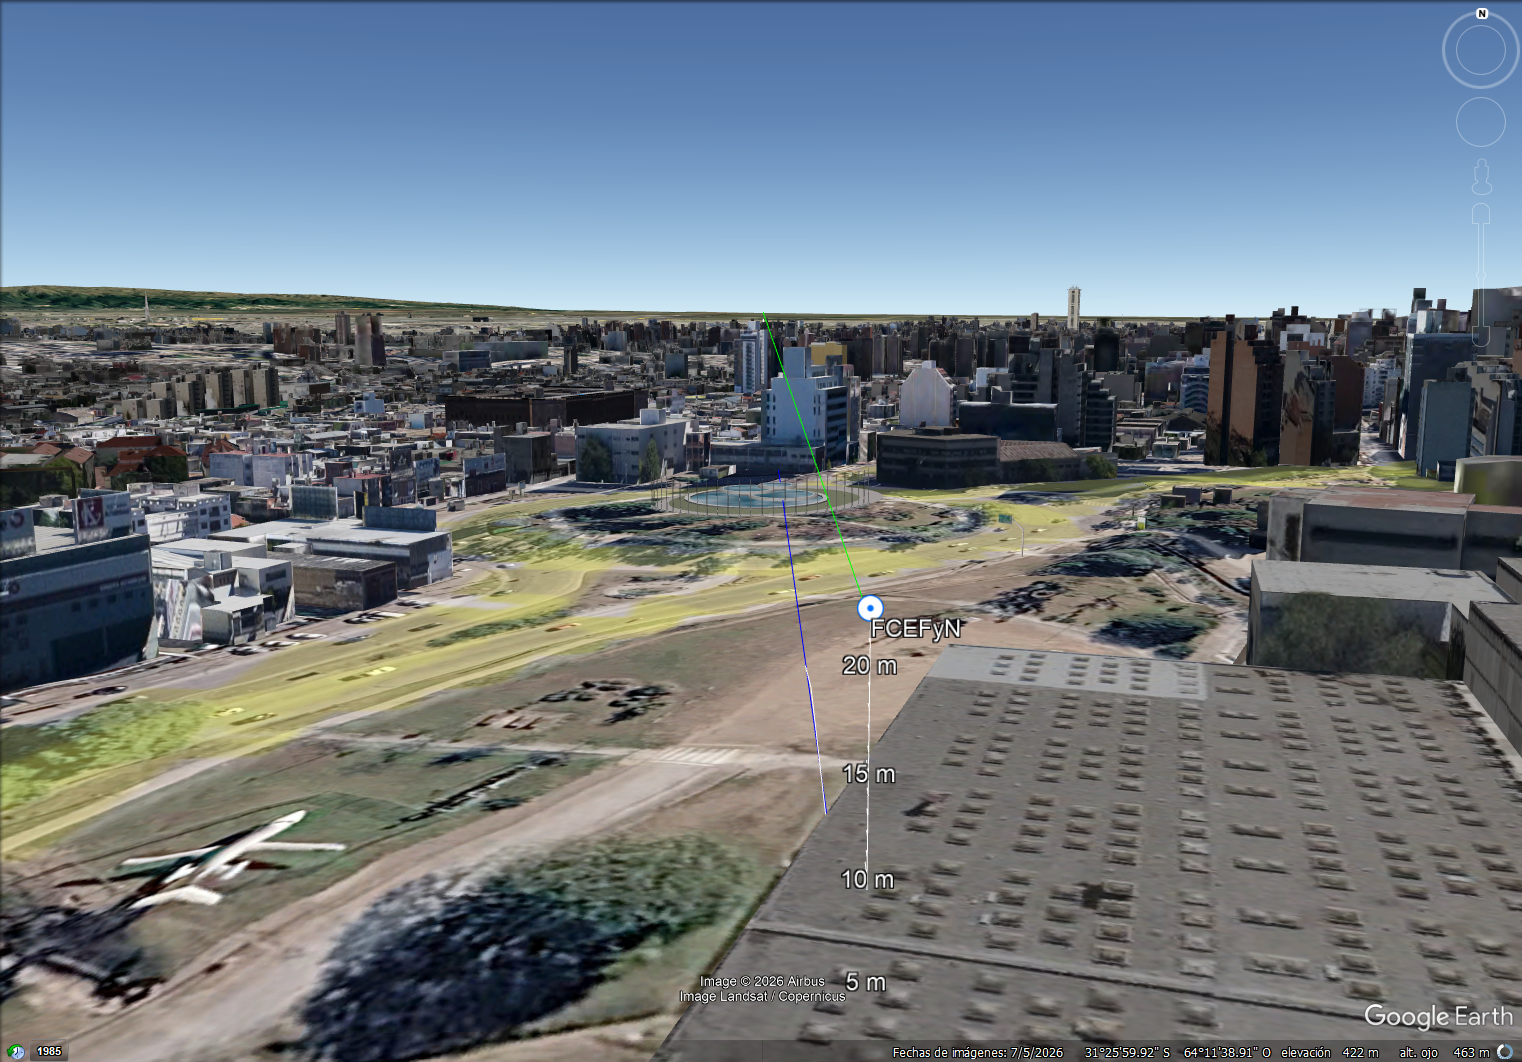
\includegraphics[width=1\linewidth]{Figura 3.1.png}
        \end{minipage}
        \hfill
        \begin{minipage}{0.48\linewidth}
            \centering
            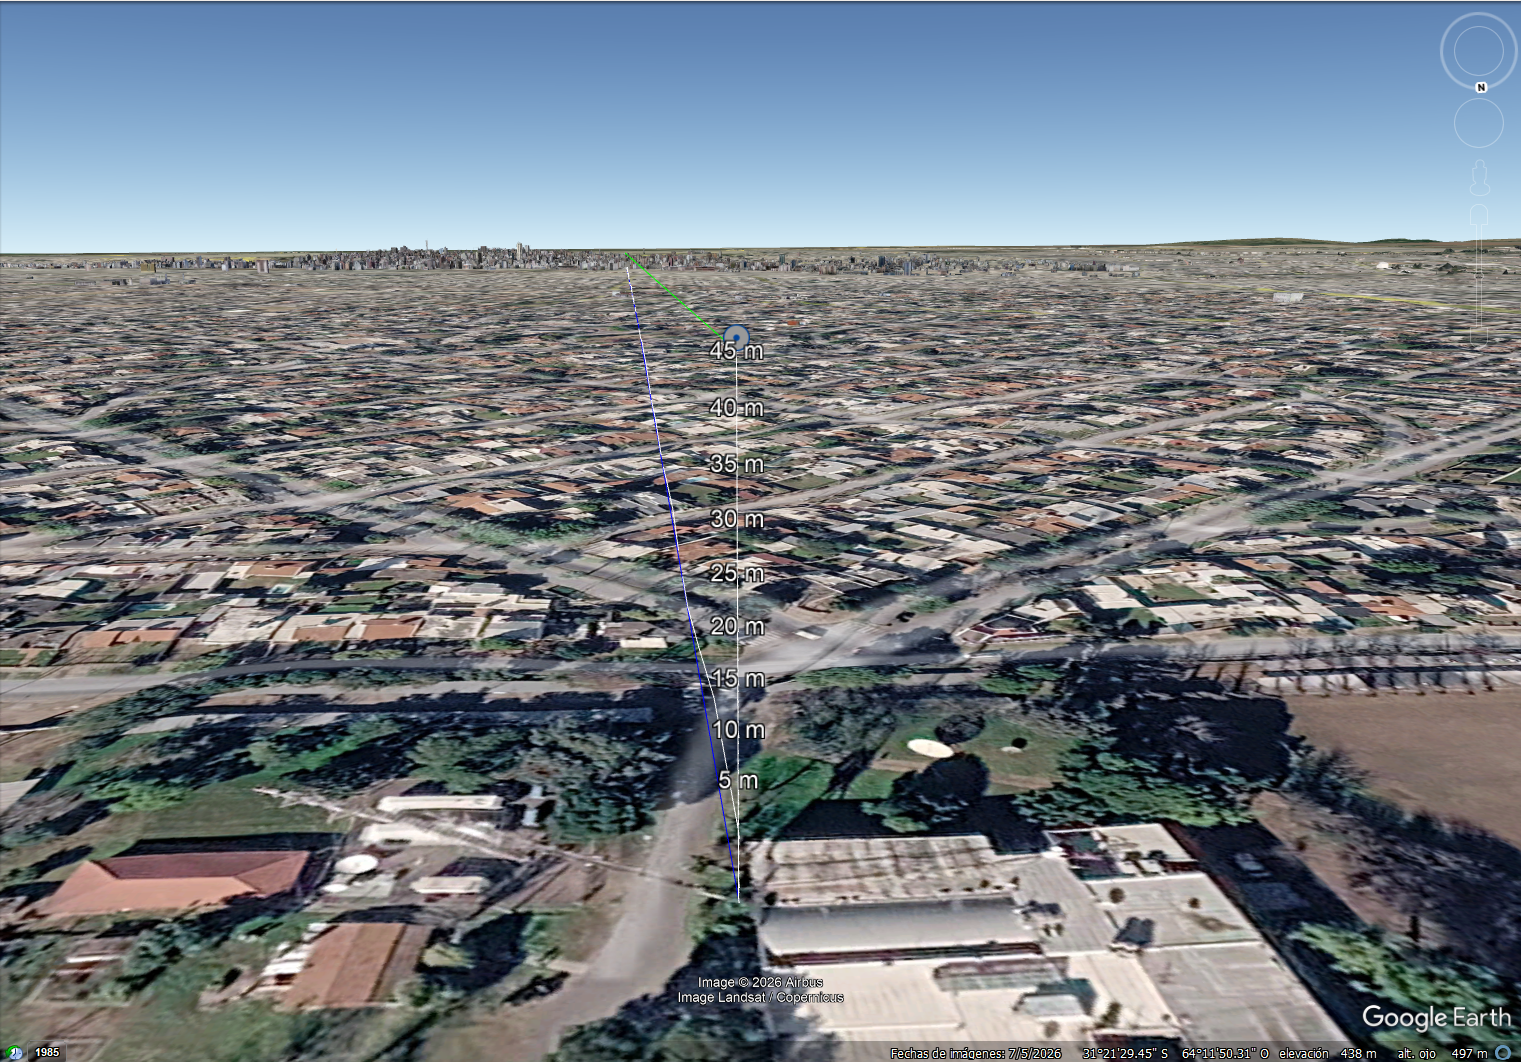
\includegraphics[width=1\linewidth]{Figura 3.2.png}
        \end{minipage}
        \caption{A la izquierda se observa el mástil de Canal 10, mientras que a la derecha se observa el avión instalado en la FCEFyN.}
        \label{fig:fig_3}
    \end{figure}

    
    \item \underline{Cálculo manual del radio de Fresnel:} El radio de Fresnel se calcula según \autoref{eq_1}. 
    \begin{equation}
        R_{F} = 17.32 \sqrt{\frac{d_{1} \cdot d_{2}}{f \cdot d}}
        \label{eq_1}
    \end{equation}

    El punto más crítico para el radio de la primera zona de Fresnel se ubica en el centro exacto del vano de $8.72 \, [km]$, es decir, a $d_{1} = d_{2} = 4.36 \, [km]$. Dado que el enlace opera a una frecuencia de operación típica de $f = 5.8 \, [GHz]$, el radio máximo ($R$) se calcula empleando la siguiente ecuación:
    \begin{equation}
        R = 17.32 \sqrt{\frac{4.36 \cdot 4.36}{5.8 \cdot 8.72}} = 10.61 \, [m]
        \label{eq_2}
    \end{equation}
    
    \item \underline{Análisis de obstáculos (punto crítico):} Observando el terreno subyacente a la línea de vista en la \autoref{Pruebas de latencia} 
    
    El edificio urbano situado a 5.35 km del origen se mantiene como la estructura más cercana a la trayectoria geométrica. No obstante, gracias al incremento en las alturas de los mástiles, la evaluación mediante Google Earth permite estimar que el haz principal transcurre a una distancia lateral y vertical lo suficientemente alejada de la edificación[cite: 4]. 
    
    \item \underline{Conclusión de despeje:} El ajuste de alturas asegura que el trayecto cumple satisfactoriamente con el requisito de mantener un despeje del 60\% o superior de la primera zona de Fresnel[cite: 4]. Al estar libre de obstrucciones e invasiones significativas, se elimina el riesgo de atenuaciones por difracción, garantizando las condiciones teóricas para alcanzar la señal esperada de -72 dBm.
\end{itemize}




\subsection{Determinación de las alturas mínimas de antena}
\label{sec_2.6}
...



\subsection{Selección de frecuencia y ancho de canal}
\label{sec_2.7}
...



\subsection{Selección del equipamiento}
\label{sec_2.8}
...



\subsection{Capacidad requerida}
\label{sec_2.9}
...



\subsection{Atenuación de espacio libre}
\label{sec_2.10}
...



\subsection{Presupuesto de radiofrecuencia}
\label{sec_2.11}
...



\subsection{PIRE}
\label{sec_2.12}
...



\subsection{Sensibilidad, modulación y margen de enlace}
\label{sec_2.13}
...



\subsection{Nivel de ruido y SNR}
\label{sec_2.14}
...



\subsection{Pérdidas adicionales y obstáculos}
\label{sec_2.15}
...



\subsection{Análisis de interferencias}
\label{sec_2.16}
...



\subsection{Consideraciones regulatorias}
\label{sec_2.17}
...



\subsection{Análisis mediante Google Earth}
\label{sec_2.18}
...



\subsection{Orientación de las antenas}
\label{sec_2.19}
...



\subsection{Sistema de montaje}
\label{sec_2.20}
...



\subsection{Cableado, alimentación y protección}
\label{sec_2.21}
...



\subsection{Optimización del enlace}
\label{sec_2.22}
...






\section{Parte 2 - Implementación y experimentación con un enlace de corta distancia}
\label{sec_3}
\subsection{Reconocimiento del equipamiento}
\label{sec_3.1}
En esta primera etapa experimental se realizó el inventario, reconocimiento e inspección técnica de los componentes disponibles en el laboratorio para el armado y puesta en marcha del enlace radioeléctrico punto a punto de corta distancia. Se reconocieron los siguientes elementos:

\begingroup
\footnotesize
\begin{longtable}
    {|>{\centering\arraybackslash}m{2cm}
     |>{\centering\arraybackslash}m{2.5cm}
     |>{\centering\arraybackslash}m{3cm}
     |>{\centering\arraybackslash}m{3.9cm}
     |>{\centering\arraybackslash}m{2.9cm}|} \hline
    \textbf{Elemento} & \textbf{Modelo} & \textbf{Función} & \textbf{Características Principales} & \textbf{Formas de Conexión} \\ \hline
    \endfirsthead
    
    \multicolumn{5}{c}{\textit{Continuación de la página anterior}} \\ \hline
    \textbf{Elemento} & \textbf{Modelo} & \textbf{Función} & \textbf{Características Principales} & \textbf{Formas de Conexión} \\ \hline
    \endhead
    
    \hline 
    \multicolumn{5}{c}{\textit{Continúa en la página siguiente...}} \\
    \endfoot
    
    \hline
    \caption{Reconocimiento de equipo incluido en el \textit{Ubiquiti LiteBeam 5AC Gen2}.}
    \label{tab:tab_3} \\
    \endlastfoot
        \textbf{Radios y Antenas (Equipo Integrado)} & 
        \textit{Ubiquiti LiteBeam 5AC Gen2}&
        Actuar como transceptor de radiofrecuencia y antena direccional integrada para el establecimiento del enlace inalámbrico. & 
        Opera en la banda de $5 \, [GHz]$ con una ganancia de $23 \, [dBi]$ en reflector parabólico. Utiliza el protocolo propietario \textit{airMAX ac} (basado en \textit{TDMA}) e integra un radio secundario de gestión en $2,4 \, [GHz]$ para configuración mediante la aplicación \textit{UISP}. & 
        Posee un puerto \textit{RJ45} blindado en la parte posterior por donde recibe simultáneamente la energía eléctrica (\textit{PoE}) y el tráfico de datos. \\ \hline


        \textbf{Fuentes e Inyectores \textit{PoE}} &
        Adaptador \textit{PoE Gigabit Ubiquiti} ($24 \, [V_{DC}]$, $0,3 \, [A]$). &
        Suministrar energía eléctrica al transceptor a través del cable de par trenzado, permitiendo la coexistencia de alimentación y datos en la misma infraestructura de cableado. &
        Salida de $24 \, [V_{DC}]$, $0,3 \, [A]$, compatibilidad con enlaces \textit{Gigabit Ethernet} y puerto con protección contra descargas electrostáticas (\textit{ESD}). &
        Alimentado desde la red eléctrica ($220 \, [V_{CA}]$). El puerto rotulado como \textit{POE} se conecta a la antena \textit{LiteBeam}, mientras que el puerto \textit{LAN} se vincula al puerto \textit{Ethernet} de la computadora. \\ \hline
        

        \textbf{Cableado y Conectores} &
        Cable de par trenzado Categoría $5e$ con conectores \textit{RJ45} blindados (con cuerpo metálico). &
        Interconectar la fuente de alimentación \textit{PoE} y el equipo terminal de datos. &
        Presencia de malla de blindaje e hilo de drenaje para la derivación de interferencias electromagnéticas (\textit{EMI}) y cargas estáticas a tierra. Velocidad de hasta $1 \, [Gbps]$ y $100 \, [MHz]$ de ancho de banda. &
        Conectores \textit{RJ45} crimpeados bajo norma \textit{T568B} en ambos extremos. \\ \hline


        \textbf{Soportes de Montaje} &
        Herraje para trípode articulado con control de altura. Montaje de acimut y montaje de elevación&
        Brindar sustentación mecánica rígida y permitir la orientación precisa del haz en altura, acimut y elevación. &
        - &
        Ensamble mecánico a la estructura de la antena y fijación al mástil mediante abrazadera metálica de ajuste. \\ \hline


        \textbf{Computa- \newline -doras de Prueba} &
        Dos computadoras portátiles (\textit{PC} Estación \textit{A} y \textit{PC} Estación \textit{B}). &
        Acceso a la interfaz de gestión \textit{airOS 8}, configuración de parámetros de red y ejecución de software para generación/medición de tráfico. &
        - &
        Interfaz de red \textit{Ethernet RJ45} conectada mediante \textit{patch cord} directo hacia el puerto \textit{LAN} del inyector \textit{PoE} correspondiente. \\ \hline

        \textbf{Instrumen- \newline -tos y Software de Medición} &
        Sistema operativo \textit{airOS 8}, analizador de espectro de \textit{RF} en tiempo real \textit{airView}, utilidad de medición de rendimiento \textit{iPerf3} y comandos de red del sistema (\textit{ping}). &
        Diagnostico del espectro radioeléctrico, medición del nivel de señal recibida (\textit{RSSI}), nivel de ruido, \textit{SNR}, tasa de transferencia útil (\textit{throughput}), latencia, \textit{jitter} y pérdida de paquetes. &
        - &
        Cinta métrica para la medición de la distancia física entre antenas en el laboratorio. \\ \hline
\end{longtable}
\endgroup

                %\autoref{fig:fig_3.1.1}
Se muestra en la                        , se muestra una captura del equipamiento y el área de trabajo:

%\begin{figure}[H]
%    \centering
%    
\includegraphics[width=0.85\textwidth]{Figura 3.1.1}
%    \caption{Inventario del equipamiento \textit{Ubiquiti LiteBeam 5AC Gen2} e instrumentos de laboratorio.}
%    \label{fig:fig_3.1.1}
%\end{figure}



\subsection{Montaje del enlace}
\label{sec_3.2}
...



\subsection{Configuración básica}
\label{sec_3.3}
...



\subsection{Análisis del espectro}
\label{sec_3.4}
...



\subsection{Alineación y ajuste fino}
\label{sec_3.5}
...



\subsection{Potencia de transmisión}
\label{sec_3.6}
...



\subsection{Pruebas de latencia}
\label{sec_3.7}
...



\subsection{Pruebas de throughput con iPerf3}
\label{sec_3.8}
...



\subsection{Prueba complementaria con Speedtest}
\label{sec_3.9}
...



\subsection{Variación del ancho de canal}
\label{sec_3.10}
...



\subsection{Introducción de una obstrucción}
\label{sec_3.11}
...



\subsection{Análisis de resultados}
\label{sec_3.12}
...



\subsection{Comparación entre teoría, simulación y medición}
\label{sec_3.13}
...



\subsection{Consideraciones sobre enlaces reales}
\label{sec_3.14}
...






\section{Conclusiones}
\label{sec_4}
...



\newpage
\printbibliography[heading=bibintoc, title={5. \, Bibliografía y Referencias}]
\end{document}
